

%L'apparato sperimentale attualmente in uso ai LNS-INFN nell'ambito della Fase~2 del progetto NUMEN, costituito principalmente dallo spettrometro MAGNEX e dal Ciclotrone Superconduttore K800, viene brevemente illustrato nella prima parte di questo capitolo.
L'apparato sperimentale attualmente in uso ai LNS-INFN nell'ambito della Fase~2 del progetto NUMEN è costituito principalmente dallo spettrometro MAGNEX e dal CS.
Poiché la descrizione di tale apparato non costituisce l'argomento primario del presente lavoro di tesi, nella prima parte del capitolo ne vengono discusse soltanto le caratteristiche principali, rimandando alla vasta letteratura sul tema per informazioni più dettagliate (ad esempio~\cite{cavallaro:epja12, carbone:epja12, cappuzzello:epja16, cunsolo:epjst07}).

%Nella prima parte di questo capitolo vengono illustrate le principali caratteristiche dell'apparato sperimentale attualmente in uso ai LNS-INFN nell'ambito della Fase~2 del progetto NUMEN.
%Nella seconda parte viene descritta la configurazione dell'apparato adottata in occasione del test sui telescopi SiC-CsI svolto ad Aprile 2018, sottolineando le differenze rispetto a quella consueta.
(\textcolor{red}{Sistemare questa parte})Nella seconda parte \textcolor{red}{si parla} del test sui telescopi SiC-CsI svolto ad Aprile~2018, esponendone le motivazioni, descrivendo la configurazione dell'apparato adottata e sottolineandone le differenze rispetto a quella consueta.


\section{\iflanguage{italian}{Lo spettrometro magnetico MAGNEX}{MAGNEX magnetic spectrometer}}

Lo spettrometro magnetico MAGNEX è un dispositivo ottico a grande accettanza costituito da un quadrupolo per la focalizzazione sull'asse verticale, seguito da un dipolo per la dispersione sul piano orizzontale.
Grazie alle sue peculiarità,  MAGNEX riesce ad offrire, in un angolo solido molto grande e in un ampio range energetico, un'ottima risoluzione in energia, angolo e massa.
Ciò lo rende uno strumento ideale per l'analisi di eventi caratterizzati da sezioni d'urto molto basse, come è già stato dimostrato in~\cite{cappuzzello:epja16,pereira:plb12,oliveira:jpg13}.
Inoltre, esso consente di effettuare misure fino a zero gradi, comprendendo, dunque, la regione angolare di massimo interesse per lo studio del DCE.

La caratteristica che rende MAGNEX uno strumento unico è l'implementazione di una innovativa tecnica di ricostruzione delle traiettorie degli ioni, che consente di correggere le inevitabili aberrazioni originate dalla grande accettanza del dispositivo.
Dunque, a differenza di altri spettrometri magnetici, per MAGNEX è importante determinare non soltanto il punto di impatto sul piano focale ma anche la traiettoria completa. Ciò significa che è necessario misurare quattro parametri: una coppia, chiamata $(x_{foc}, y_{foc})$, individua il punto di impatto, l'altra, indicata con $(\theta_{foc}, \phi_{foc})$, si riferisce rispettivamente all'angolo orizzontale e a quello verticale.
%Nel paragrafo successivo verrà esplicato in che modo vengono misurati tali parametri.
Il modo in cui tali parametri vengono misurati sarà esplicato nel paragrafo successivo.

In Figura~\ref{fig:magnex} è mostrata una foto di MAGNEX, in cui è possibile notare, andando da sinistra verso destra, la camera di scattering, il quadrupolo, il dipolo e il~FPD (\textcolor{red}{Aggiungere le scritte sull'immagine}).

\begin{figure} [!t]
	\centering
	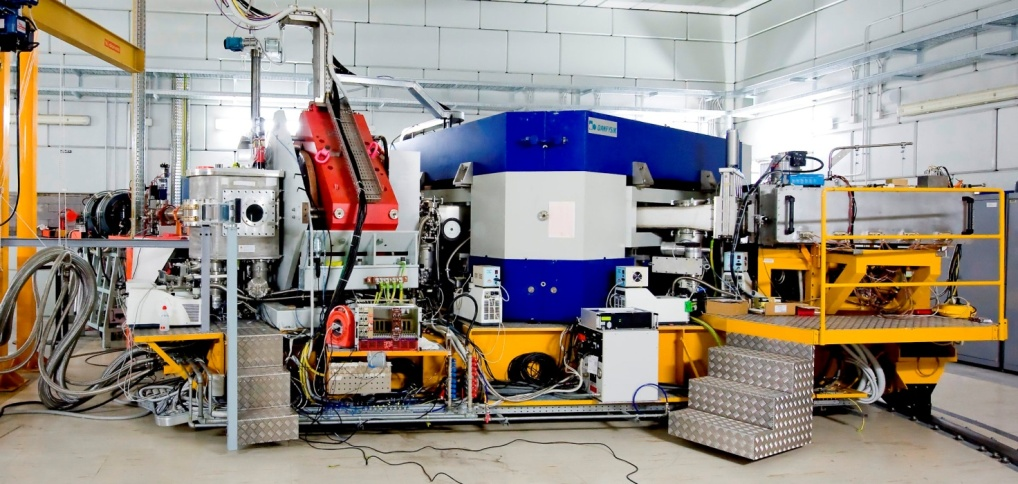
\includegraphics[width=\textwidth, keepaspectratio]{Grafici/magnex.jpg}
	\caption{Lo spettrometro magnetico MAGNEX.} \label{fig:magnex}
\end{figure}



%\clearpage 

\subsection{\iflanguage{italian}{Il rivelatore di piano focale}{The Focal Plane Detector}} \label{sez:fpd}

\begin{figure} [!p]
	\centering
	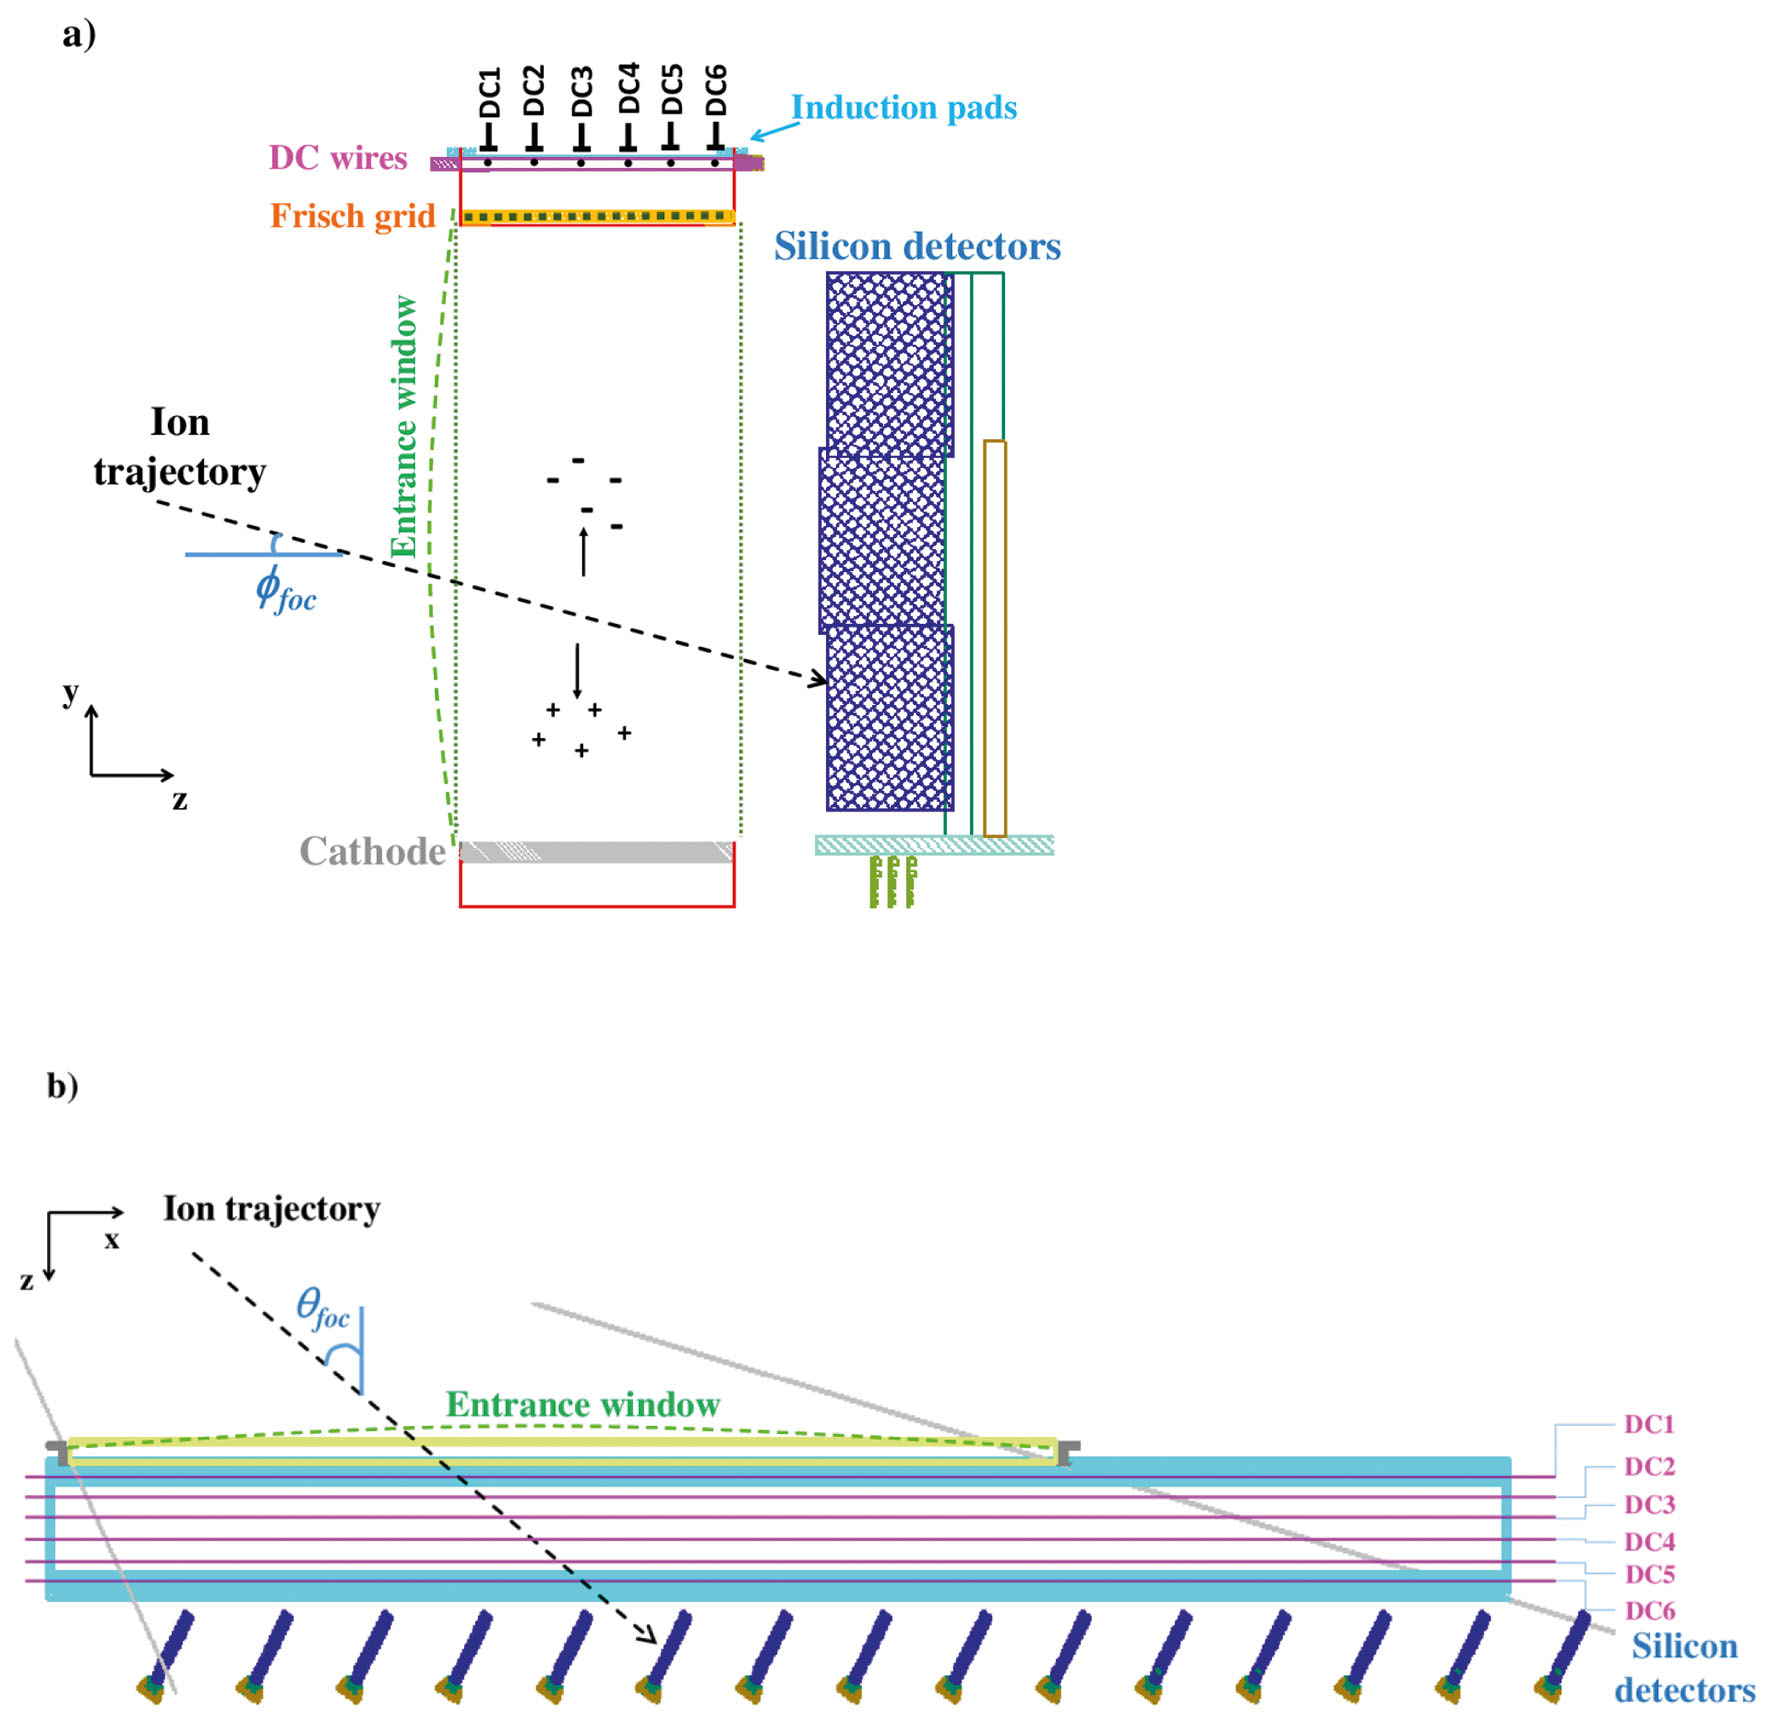
\includegraphics[width=\textwidth, keepaspectratio]{Grafici/fpd.png}
	\caption{Rappresentazione schematica del FPD: a) vista laterale; b) vista dall'alto. Figura tratta da~\cite{cappuzzello:epja18}.} \label{fig:fpd}
\end{figure}

L'attuale FPD di MAGNEX, la cui rappresentazione schematica è riportata in Figura~\ref{fig:fpd}, è un sistema di rivelazione ibrido, costituito da un tracciatore a gas a bassa pressione e da un muro di rivelatori al silicio.
Esso è posizionato a 1.91~m dall'uscita del dipolo e, al fine di minimizzare gli effetti dovuti alle aberrazioni cromatiche\cite{cunsolo:nima01}, è inclinato di 59.2\textdegree{} rispetto ad un piano perpendicolare all'asse ottico.
Una finestra di mylar spessa 1.5~$\mu$m è utilizzata per contenere il gas, solitamente costituito da N35 isobutano, segnando l'ingresso nel volume attivo.




%Il tracciatore a gas è formato da un sistema di sei fili al tungsteno placcati in oro, posti al di sotto di un anodo segmentato in pad. 
%Il tracciatore a gas lavora secondo il principio tipico delle camera a deriva.
%Il tracciatore a gas è essenzialmente una camera a deriva, in cui un sistema misto di fili e pad consente la misura dei quattro parametri necessari.
%Il tracciatore a gas, che consente la ricostruzione tridimensionale della traiettoria degli ioni, è formato da sei fili al tungsteno, indicati con DC\ped{\textit{i}}, e da un anodo segmentato in pad. 
%Al di sopra di ciascun filo si trova una fila di 224 pad
%Il tracciatore a gas è essenzialmente una camera a deriva, in cui un sistema costituito da sei fili (DC\ped{\textit{i}}) e da un anodo segmentato in pad consente la misura dei quattro parametri necessari per la ricostruzione tridimensionale della traccia.
%In particolare, al di sopra di ciascun filo è presente una fila di pad, le quali sono orientate parallelamente all'asse ottico.
Il tracciatore a gas, che consente la ricostruzione tridimensionale della traiettoria degli ioni, è formato da sei fili proporzionali (DC\ped{\textit{i}}) e da un anodo segmentato in sei file di pad, disposti in modo che sopra ogni filo ci sia una fila di pad.
I fili, sfruttando il principio di lavoro delle camere a deriva, danno una misura di sei posizioni verticali ($Y_i$), mentre le pad permettono di determinare sei posizioni orizzontali ($X_i$).
%Una griglia di Frisch è posta al di sotto dei fili, in quanto questi vengono anche utilizzati per misurare l'energia persa dagli ioni nel gas.
Dal momento che i fili vengono anche utilizzati per misurare l'energia persa dagli ioni nel gas, una griglia di Frisch è posta al di sotto di essi.




Il muro di rivelatori al silicio è formato da 60 pad, organizzate in 20 colonne da 3 rivelatori ciascuna. (\textcolor{red}{Aggiungo qualche dettaglio in più?})
%Ogni pad ha un'area attiva di $70 \times 50$~mm\ap{2} ed è spessa 500~$\mu$m, sufficienti per fermare i prodotti di reazioni nel range energetico di interesse. 
Essi vengono utilizzati per fermare gli ioni, misurandone l'energia residua e producendo il segnale di trigger per l'acquisizione. 

Quando una particella carica, attraversando la finestra di mylar, entra nel volume attivo, produce nel gas coppie elettrone-ione positivo, le quali, sotto l'effetto di un campo elettrico costante, migrano rispettivamente verso la griglia di Frisch e il catodo. 
%mentre gli elettroni diffondono verso la griglia di Frisch, con una velocità che per questi ultimi è di circa $3 - 5 $~cm/$\mu$s. 
%La presenza di un campo elettrico costante provoca 
%La velocità di deriva tipica degli elettroni è di $3 - 5 $~cm/$\mu$s
Dopo aver attraversato la griglia, gli elettroni giungono in prossimità dei fili DC\ped{\textit{i}}, dove, a causa dell'elevato campo elettrico, danno luogo alla moltiplicazione a valanga. 
%La carica prodotta, proporzionale all'energia persa dalla particella nel gas, induce sulle pad una distribuzione di carica, della quale si calcola il baricentro. Questa operazione avviene per le sei file di pad, in modo tale che ai sei baricentri corrispondono sei misure di posizioni orizzantali $X_i$.
Alle tensioni e pressioni utilizzate, la carica secondaria prodotta genera un segnale proporzionale all'energia persa dalla particella nel gas. 
Poiché ciò avviene per ciascuno dei sei fili, si hanno sei segnali di perdita di energia, indicati con~$\Delta E_i$.

La stessa valanga induce sulle pad una distribuzione di carica, di cui si calcola, tramite un apposito software, il centro di gravità. Anche in questo caso l'operazione si ripete per le sei file di pad, così che vengono estratte sei misure di posizioni orizzontali~$X_i$.
A questo punto, effettuando un fit lineare sulle sei posizioni~$X_i$, si ottengono $x_{foc}$ e $\theta_{foc}$ rispettivamente dall'intercetta e dal coefficiente angolare della retta.

Superata la regione del tracciatore, la particella carica arriva al muro dei rivelatori al silicio, dove si ferma producendo un segnale proporzionale alla sua energia residua~$E_{resid}$. 
Lo stesso segnale viene utilizzato per calcolare l'intervallo di tempo impiegato dagli elettroni primari prodotti nel gas per raggiungere i fili DC\ped{\textit{i}}. 
%Dal momento che tale intervallo è proporzionale allo spazio percorso, si ottengono così sei misure di posizioni verticali~$Y_i$, dalle quali, grazie ad un fit lineare, si ricavano $y_{foc}$ e $\phi_{foc}$ in maniera analoga a quanto visto per $x_{foc}$ e $\theta_{foc}$.
Dal momento che la velocità di deriva è costante, tale intervallo di tempo è direttamente proporzionale allo spazio percorso. Si ottengono, dunque, sei misure di posizioni verticali~$Y_i$, dalle quali, grazie ad un fit lineare, si ricavano $y_{foc}$ e $\phi_{foc}$ in maniera analoga a quanto visto per $x_{foc}$ e $\theta_{foc}$.

È bene ricordare che, nelle camere a deriva a fili, la maggior parte del segnale è originata dal moto degli ioni positivi e non degli elettroni.
Di conseguenza, a causa della minore velocità degli ioni, tale tipologia di rivelatori può tipicamente sostenere rate dell'ordine di pochi~kHz. 
Questo aspetto, che costituisce una delle principali limitazioni all'intensità del fascio tollerabile dall'attuale FPD, deve essere superato nell'ottica della Fase~4. 
Nasce da qui l'esigenza di sostituire l'attuale tracciatore con un sistema in grado di lavorare con un rate elevato di ioni pesanti. 




\section{\iflanguage{italian}{Il test sui telescopi SiC-CsI}{Experimental setting for the test}}

%Ad Aprile 2018 è stato svolto un test sui primi due prototipi di telescopi SiC-CsI, allo scopo di confrontarne la risposta con il sistema attualmente utilizzato.
%Ad Aprile 2018 è stato svolto un test sui primi due prototipi di telescopi SiC-CsI, allo scopo di valutarne la risposta, confrontandola con quella del sistema attualmente utilizzato.

Ad Aprile 2018 i primi due prototipi di rivelatori al SiC per il progetto NUMEN sono stati completati e resi disponibili dalla \textcolor{red}{ST-Microelectronics} (\textcolor{red}{giusto?}).
%Dopo aver realizzato 
%Per verificare se la risposta di un telescopio formato da uno stadio $\Delta E$ al SiC seguito da un cristallo di CsI poteva garantire prestazioni di identificazione degli ioni confrontabili con quelle accessibili con l'attuale apparato, è stato svolto un test per una durata complessiva di cinque giorni.
%Dal momento che tali rivelatori non sono ancora uno standard nel mondo della fisica ma rappresentano una tecnologia nuova, è stato svolto un test per verificare se le loro prestazioni possono soddisfare le esigenze di NUMEN.
Dal momento che tali rivelatori non sono ancora uno standard nel mondo della fisica ma rappresentano una tecnologia di frontiera, è stato condotto un test per analizzarne la risposta nelle condizioni sperimentali tipiche della Fase~2 di NUMEN.
%Come illustrato nel Paragrafo~\ref{sez:sistema_identif_part}, i rivelatori al SiC sono stati scelti nell'ambito del progetto per assolvere al ruolo di sistema di PID
%Sono stati, dunque, assemblati due telescopi SiC-CsI, di cui si è studiata la risposta in termini di PID.
Come illustrato nel Paragrafo~\ref{sez:sistema_identif_part}, i rivelatori al SiC sono stati scelti nell'ambito del progetto come stadio~$\Delta E$ di un telescopio SiC-CsI per l'identificazione in numero atomico dei prodotti di reazione.
%Come illustrato nel Paragrafo~\ref{sez:sistema_identif_part}, i rivelatori al SiC sono stati scelti nell'ambito del progetto per identificare i prodotti di reazione
Lo scopo principale del test era, dunque, valutare la capacità di PID di questo sistema nella regione di interesse per NUMEN, confrontandola con quella accessibile con l'attuale apparato.

%Il fascio utilizzato nel test era costituito da \ce{^{20}Ne}, mentre i bersagli erano \ce{^{197}Au} e \ce{^{12}C}
Il test è stato svolto utilizzando un fascio di~\ce{^{20}Ne} a 20~MeV/u, incidente su \ce{^{197}Au} o \ce{^{12}C}, laddove i due bersagli avevano funzioni differenti: il primo serviva per la localizzazione dello scattering elastico, il secondo per favorire la formazione dei prodotti di reazione di interesse per NUMEN, ovvero O, F~e~Ne.






%\subsection{\iflanguage{italian}{I telescopi SiC-CsI}{SiC-CsI telescope detectors}}

\subsection{\iflanguage{italian}{I rivelatori al carburo di silicio}{Silicon carbide detectors}}


%I dispositivi al SiC costituiscono oggi una promettente realtà nel campo dei rivelatori per la fisica, 
Grazie alle sue interessanti proprietà, il SiC costituisce oggi una promettente realtà nel campo della realizzazione di rivelatori per la fisica, configurandosi come una potenziale alternativa al silicio nelle applicazioni che richiedono una grande resistenza alle radiazioni.
La larghezza della sua gap, quasi doppia rispetto a quella del silicio, se da un lato aumenta l'energia media per la produzione di una coppia elettrone-lacuna, dall'altro riduce il numero di portatori di carica generati per agitazione termica, mantenendo, dunque, un ottimo rapporto segnale-rumore. 
Recenti test\cite{tudisco:sensors18} hanno dimostrato che con un rivelatore da 100~$\mu$m è possibile ottenere una risoluzione energetica dello 0.8\%~FWHM per le particelle $\alpha$ dell'\ce{^{241}Am} a 5486~keV.

Come la maggior parte dei rivelatori a semiconduttore, i rivelatori al SiC sono costituiti da una giunzione p-n, polarizzata inversamente per aumentare l'estensione della regione svuotata e per migliorare l'efficienza di raccolta dei portatori di carica.
Quando una particella carica attraversa il rivelatore, perde energia generando coppie elettrone-lacuna, le quali, in presenza di un campo elettrico, si muovono verso gli elettrodi, producendo il segnale.



%I due prototipi di rivelatori al SiC utilizzati nel test sono mostrati in Figura~\ref{fig:sic}; essi avevano caratteristiche differenti: uno, chiamato \emph{SiC~A}, aveva un'area attiva non segmentata di $10 \times 10$~mm\ap{2}, con uno spessore di 10~$\mu$m ed uno strato morto di 100~$\mu$m; l'altro, indicato con \emph{SiC~B}, aveva un'area attiva segmentata in quattro pad, ciascuna di $5 \times 5$~mm\ap{2}, con uno spessore di 100~$\mu$m ed un strato morto di 350~$\mu$m.

I due prototipi di rivelatori al SiC utilizzati nel test sono mostrati in Figura~\ref{fig:sic} (\textcolor{red}{modificare figura}): come è possibile notare, essi differivano innanzitutto per la segmentazione dell'area attiva, in quanto uno, chiamato \emph{SiC~A}, era costituito da un'unica pad, mentre l'altro, indicato con \emph{SiC~B}, era suddiviso in quattro regioni. 
%Inoltre, mentre il SiC~A aveva un'area attiva di $10 \times 10$~mm\ap{2}, il SiC~B presentava 
%I due telescopi SiC-CsI utilizzati nel test
Entrambi i rivelatori avevano un'area attiva complessiva di $10 \times 10$~mm\ap{2}, laddove ogni pad del SiC~B aveva un'estensione di $5 \times 5$~mm\ap{2}.
%Un'ulteriore differenza riguardava gli spessori dei due rivelatori: mentre il SiC~A era spesso 10~$\mu$m con 100~$\mu$m di strato morto, il SiC~B aveva uno spessore di 100~$\mu$m con 350~$\mu$m di .
Un'ulteriore differenza riguardava lo spessore della regione attiva dei due rivelatori: per il SiC~A era di 10~$\mu$m, mentre per il SiC~B misurava 100~$\mu$m.
Infine, entrami i rivelatori avevano uno strato morto che, mentre per il SiC~A era spesso 100~$\mu$m, per il SiC~B aveva uno spessore di~350~$\mu$m.




\begin{figure} [!t]
	\centering
	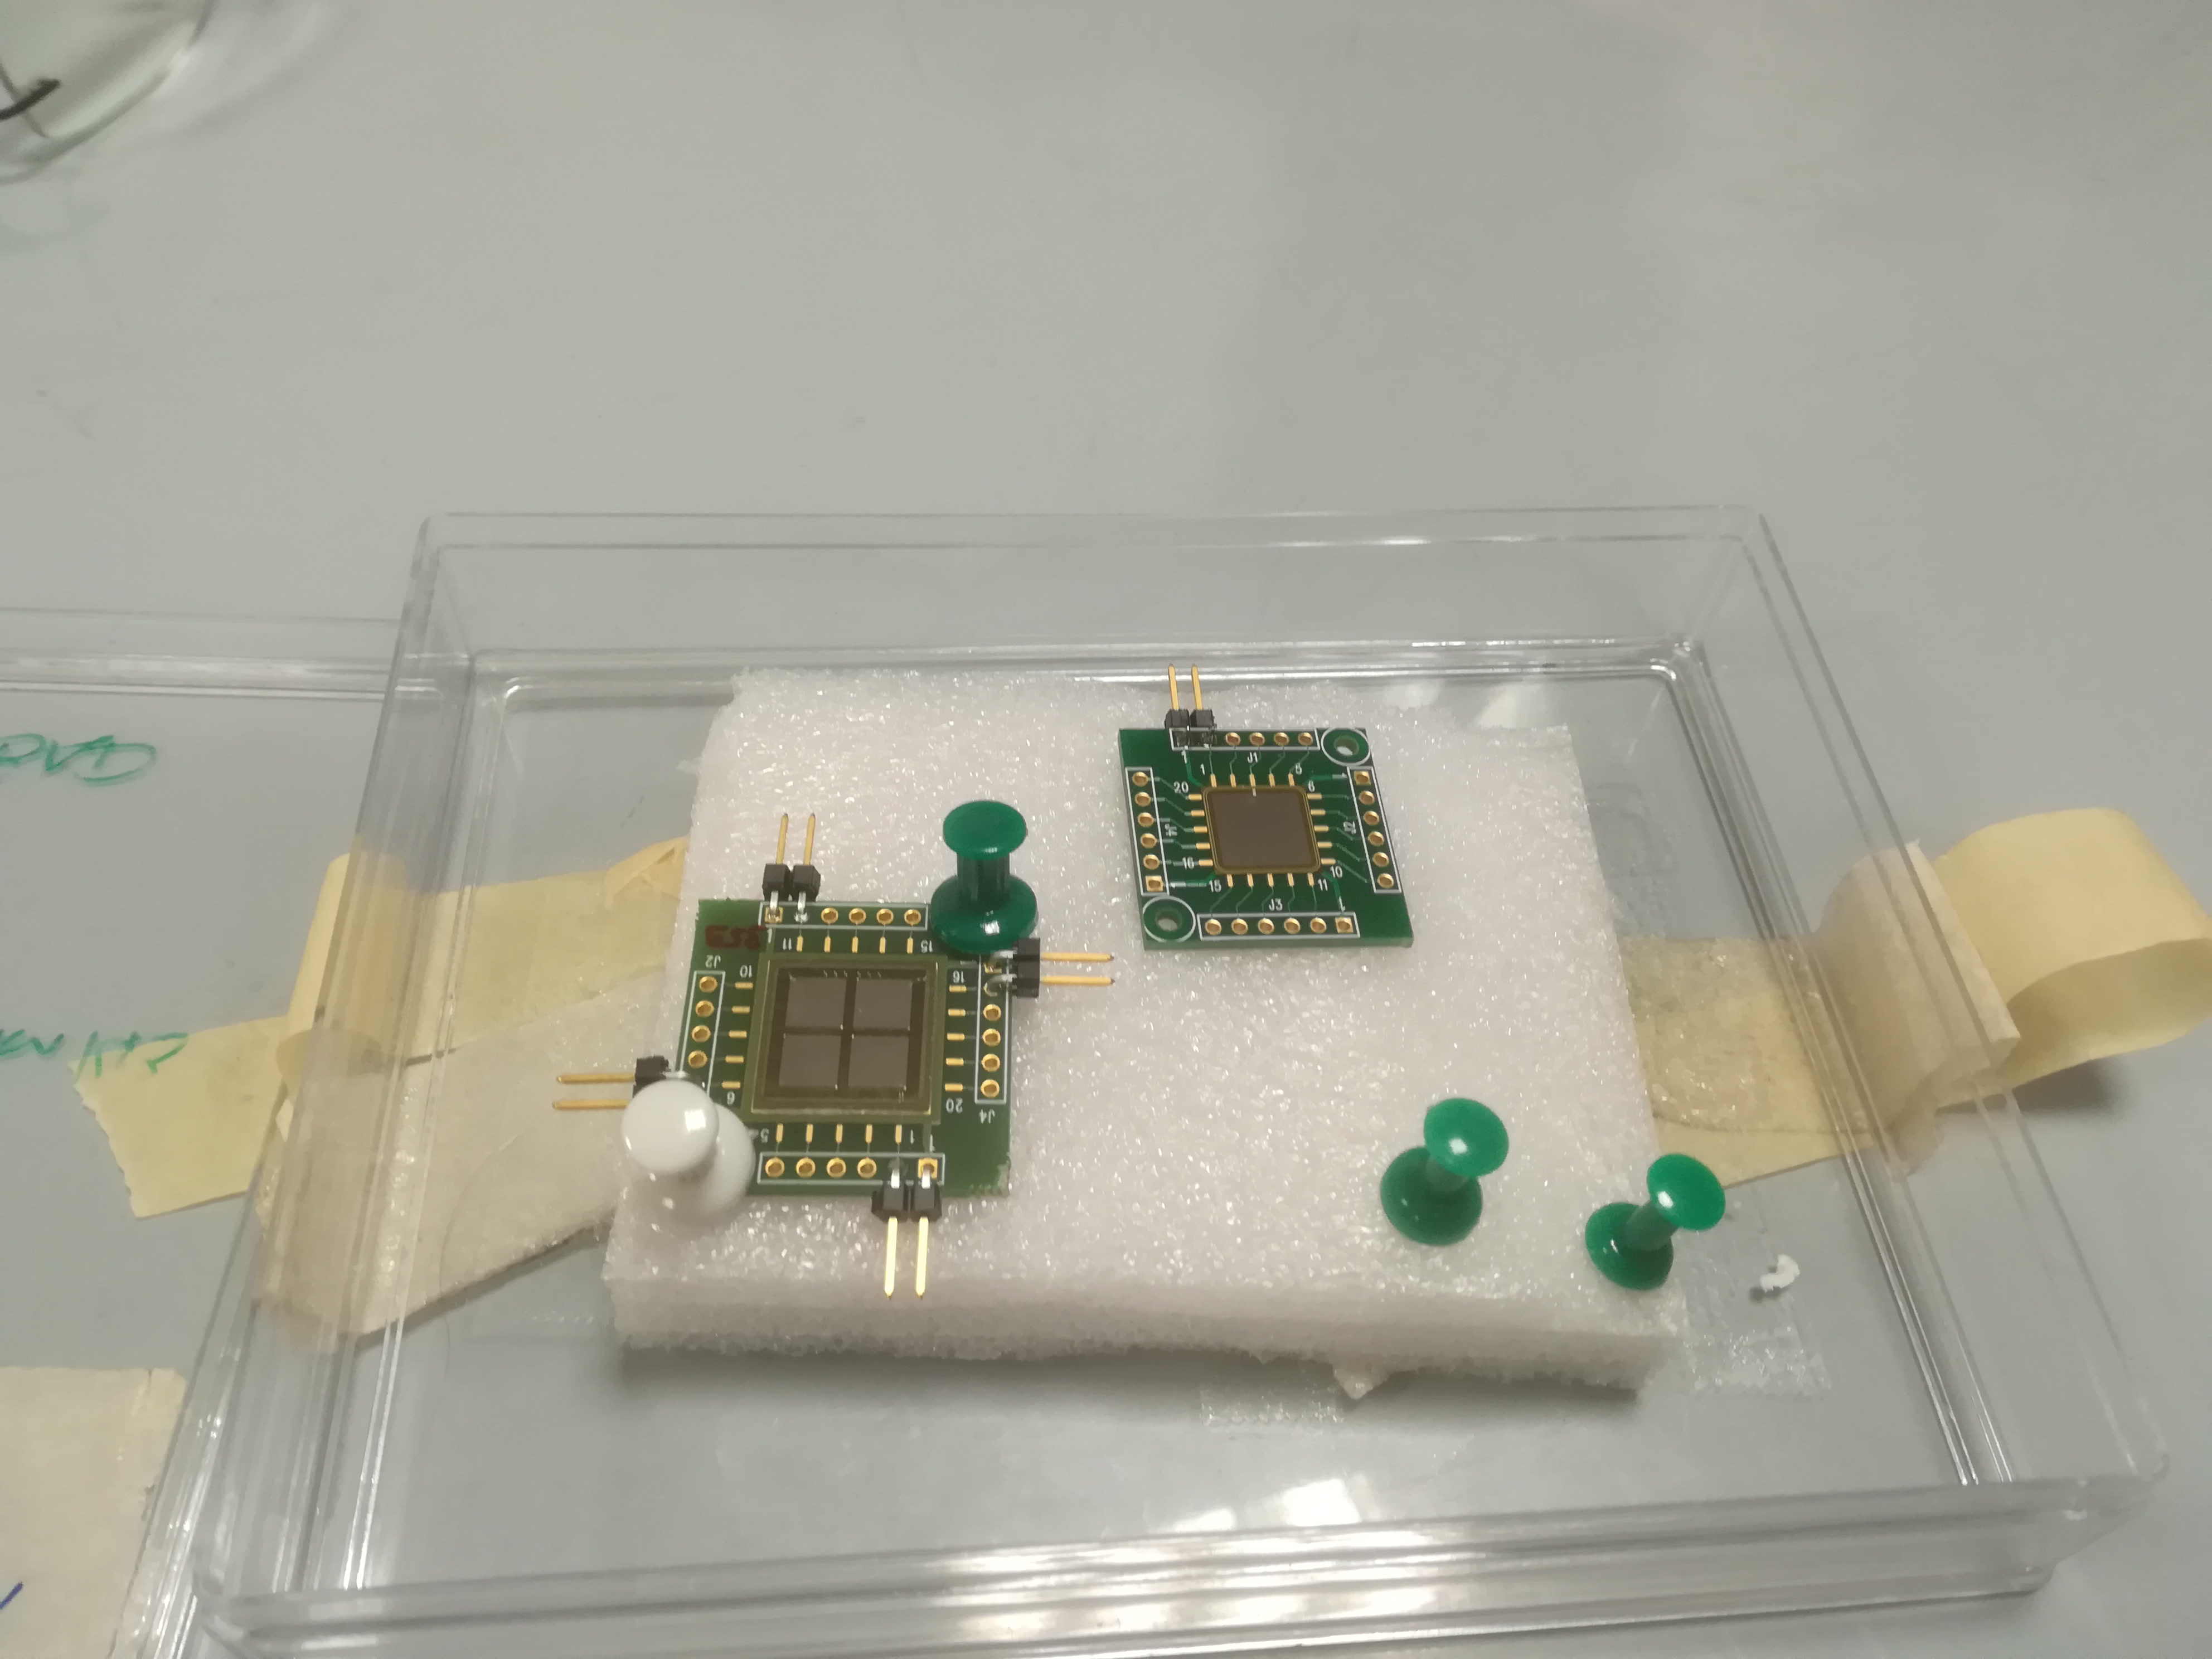
\includegraphics[width=\textwidth, keepaspectratio]{Grafici/sic.jpg}
	\caption{I rivelatori al carburo di silicio (SiC) utilizzati nel test: a sinistra quello da 100~$\mu$m, a destra quello da 10~$\mu$m.} \label{fig:sic}
\end{figure}

%I due prototipi di rivelatori al SiC utilizzati nel test presentavano caratteristiche differenti: in primo luogo avevano spessore diversi, poiché uno era spesso 10~$\mu$m, mentre l'altro 100~$\mu$m.





\clearpage

\subsection{\iflanguage{italian}{La configurazione dell'apparato sperimentale}{Experimetal apparatus setting}}

